\section{受限 Mac 实验协议与结果导入}
% chktex 24 is a false positive: this section label belongs after the heading.
\label{sec:protocol} % chktex 24

\subsection{固定实验矩阵}

正式性能证据取自固定 Mac/Colima 环境：cgroup v2 \texttt{memory.max}=2\,GiB、四个 benchmark vCPU、\texttt{memory.swap.max}=0、\texttt{pp64}、\texttt{tg16}、相同 prompt、seed 和上下文。冻结模型为 Qwen3-Next-80B-A3B-Instruct-Q4\_K\_M.gguf，文件大小为 48,410,988,384 B（约 45.09\,GiB），SHA-256 为 \texttt{d103b2733ec1012a52d01edda66b7e5c24ae50508c9f99f5297ea459ef3c061a}；冻结 llama.cpp revision 为 \texttt{360e134}。实验按 baseline、patched-control、patched-reclaim、patched-residency、patched-combined 执行；\textbf{恰好两轮}，每轮中每个配置各有一次 cold 和一次 warm，共 \FinalsResultsRunCount{} 次运行。全部运行成功，且没有用重试结果覆盖失败行。

\subsection{记录与推广门槛}

每个接受行必须绑定本地 commit、完整 patched source hash、模型 SHA-256、镜像 ID 与变体链接、资源限制、缓存标签、wall time、吞吐、cgroup peak、OOM/swap/fault/I/O 计数、运行时指标和原始运行目录。回收仅在降低稳定档位，或将 \texttt{memory.peak} 降低至少 10\% 且 wall regression 不超过 15\%、major faults 与 read bytes 不超过 control 的两倍时，才可能 promoted。驻留需在浪费、storage reads 或 decode throughput 中至少一项改善 10\%，并满足相同稳定档位与 wall regression 约束。combined 还必须优于 control 和至少一个单项最终候选。否则分类为 \texttt{kept\_opt\_in}、\texttt{rejected} 或 \texttt{insufficient\_evidence}。

\subsection{结果状态}

两轮矩阵已完成。第\ref{tab:finals-results}表显示，所有配置的聚合峰值都落在 \FinalsPeakMinimumGiB--\FinalsPeakMaximumGiB\,GiB；在该 cgroup 上限已经饱和的实验中，不能声称任何机制降低了峰值内存。cold 条件下 patched-control 相比 baseline 的 wall time 和 decode throughput 均改善，而 warm 条件下方向相反，说明缓存状态足以改变排序，不能把 cold/warm 混合为一个加速比。

单项机制呈现的是``可保留但不能推广''：reclaim 与 residency 在总体 gate 中均为 \path{kept_opt_in}。这类分类只说明它们没有越过拒绝边界，并不证明机制动作导致了表中波动。相反，combined 的 cold wall time 为 \FinalsCombinedColdWall\,s，相对 control 的 \FinalsControlColdWall\,s 回退 \FinalsCombinedColdRegressionPercent\%；cold gate 和总体决策均拒绝组合策略。这一负结果表明，两项保守策略叠加会增加 fault/admission 路径上的成本，单独看机制正确性不能推出协同收益。

JSON 的生成、核验和填表步骤记录于 \texttt{RESULTS\_IMPORT.md}。正式构建驱动每次读取固定路径 JSON，重新生成并逐字节核验 hash 绑定的 \texttt{generated\_finals\_results.tex}，然后才调用 XeLaTeX/BibTeX。第\ref{tab:finals-results}表、第\ref{tab:finals-decisions}表和本节所有数值宏都来自该导入文件。

\FinalsResultsTable
\FinalsDecisionSummary

\begin{figure}[H]
\centering
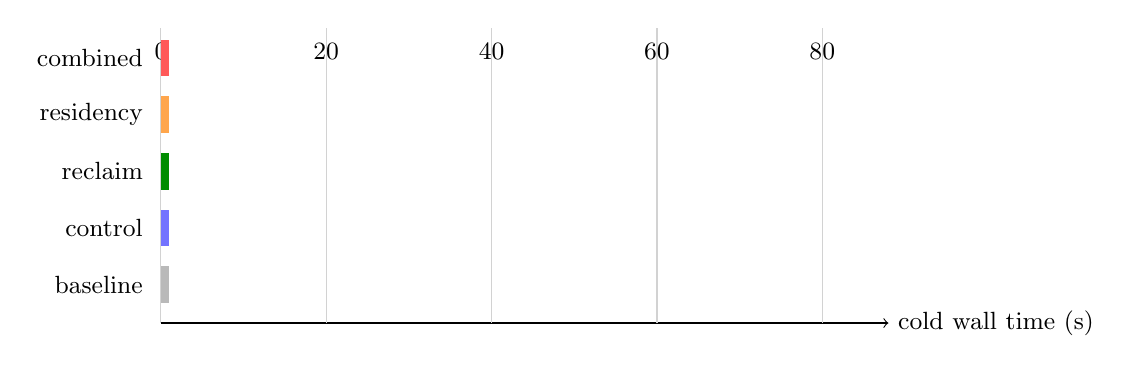
\begin{tikzpicture}[x=0.105cm,y=0.72cm,font=\small]
  \draw[->] (0,0) -- (88,0) node[right] {cold wall time (s)};
  \foreach \x in {0,20,40,60,80} {\draw[gray!35] (\x,0) -- (\x,5.2) node[below=2pt,black] {\x};}
  \fill[gray!55] (0,0.35) rectangle (\FinalsBaselineColdWall,1.00);
  \fill[blue!55] (0,1.35) rectangle (\FinalsControlColdWall,2.00);
  \fill[green!55!black] (0,2.35) rectangle (\FinalsReclaimColdWall,3.00);
  \fill[orange!70] (0,3.35) rectangle (\FinalsResidencyColdWall,4.00);
  \fill[red!65] (0,4.35) rectangle (\FinalsCombinedColdWall,5.00);
  \node[anchor=east] at (-1,0.68) {baseline};
  \node[anchor=east] at (-1,1.68) {control};
  \node[anchor=east] at (-1,2.68) {reclaim};
  \node[anchor=east] at (-1,3.68) {residency};
  \node[anchor=east] at (-1,4.68) {combined};
  \node[anchor=west] at (\FinalsBaselineColdWall+1,0.68) {\FinalsBaselineColdWall};
  \node[anchor=west] at (\FinalsControlColdWall+1,1.68) {\FinalsControlColdWall};
  \node[anchor=west] at (\FinalsReclaimColdWall+1,2.68) {\FinalsReclaimColdWall};
  \node[anchor=west] at (\FinalsResidencyColdWall+1,3.68) {\FinalsResidencyColdWall};
  \node[anchor=west] at (\FinalsCombinedColdWall+1,4.68) {\FinalsCombinedColdWall};
\end{tikzpicture}
\caption{固定 2\,GiB 协议下的 cold wall time。数值由 hash 绑定的正式 JSON 宏生成；该图用于展示配置排序和组合回退，不表示跨设备加速比。}
\label{fig:finals-cold-wall}
\end{figure}

\subsection{跨设备边界实验}

Mac 正式矩阵回答“在严格可复现的 2\,GiB 容器协议下是否应推广新机制”；RK3588 与树莓派实验回答“页建议和提前读在不同存储链路上为什么会改变方向”。三者的 CPU、文件系统、缓存边界和工作负载不同，因此表\ref{tab:edge-boundaries}只在每台设备内部做匹配比较，不计算跨设备加速比。

\begin{table}[H]
  \centering
  \scriptsize
  \caption{决赛跨设备实验及其可推广边界}
  \label{tab:edge-boundaries}
  \begin{tabular}{p{0.14\textwidth}p{0.22\textwidth}p{0.27\textwidth}p{0.21\textwidth}}
    \toprule
    环境 & 匹配实验 & 观测 & 决策 \\
    \midrule
    Mac/Colima，2\,GiB，no-swap
      & 两轮五配置 cold/warm，\texttt{pp64}/\texttt{tg16}
      & 20/20 成功；所有配置峰值均为 2\,GiB；组合策略 cold wall 回退 \FinalsCombinedColdRegressionPercent\%
      & 回收/驻留保留 opt-in；组合拒绝 \\
    RK3588，8\,GB，NVMe
      & 80B，\texttt{p32/n16/t4}；静态 RANDOM、禁用、动态阶段建议
      & 静态全开为 0.44/0.26\,t/s；禁用为 2.74/1.41\,t/s；动态策略达到 2.84/1.40\,t/s
      & Prefill 使用 SEQUENTIAL；Decode 在该设备保留预读，拒绝静态 RANDOM \\
    树莓派 5，4\,GiB，NTFS-3G/FUSE，no-swap
      & A45/A46 相邻 \texttt{pp16}：精确 expert 文件预读开/关
      & 0.0936006 对 0.0938368\,t/s，开启后为 $-0.251714\%$；没有测得 decode
      & 默认关闭文件级提前读；下一步优先减少实际专家读取量 \\
    \bottomrule
  \end{tabular}
\end{table}

RK3588 的反例揭示了机制边界：当 45.09\,GiB 权重在 8\,GB 内存中持续轮转时，静态 \path{MADV_RANDOM} 把可合并的读请求分裂为大量同步小缺页；顺序预读通过较大 I/O 摊薄内核 fault、DMA 与 SMMU 以及弱核中断路径上的固定开销。阶段感知策略恢复了 Prefill，并使 Decode 追平禁用路径。这里的结论是“策略匹配硬件”，而不是“SEQUENTIAL 在所有设备上更快”。

树莓派实验使用同一 48,410,988,384 B 模型和相邻开/关运行。\texttt{POSIX\_FADV\_WILLNEED} 只把请求提前交给 FUSE/内核，没有减少实际读取量，也没有改善 USB Bulk-Only 队列深度，因而结果中性略负。A47 对旧源码的复现与当前 control 只差 0.61\%，却无法复现历史所谓 cold 绝对值，说明仅清 Linux page cache 不能证明 FUSE、USB bridge 和 SSD 内部缓存同时为 cold；相关历史跨批次倍数不用于结论。正在探索的 expert top-$k$ 裁剪也不进入本报告性能表，除非固定质量题与原始 top-10 的匹配对照完成。
